\chapter{Evaluation}\label{Evaluation}
The evaluation is conducted to conclude whether the problem stated in this report is being solved. The answer will be acquired when the data gained from evaluation is analysed and concluded upon.
This section will attempt to evaluate the control schemes and will cover methods and different approaches planned to be used when conducting the evaluation. 
It will be discussed why usability testing methods were chosen for evaluating the prototype and why it seemed the most efficient and suitable choice. 

\section{Usability testing}
This testing method can reveal various errors that could occur when a user interacts with an interface. Usability testing is a method that seeks to test five distinct areas. \cite{usability}

\begin{itemize}
\item Efficiency\\
How quickly can the user complete certain tasks when they know the design. \cite{usability}
\item Satisfaction\\
How satisfied are the users with the design. \cite{usability}
\item Errors\\
How many errors do the users make. Is it severe errors and how quickly will they recover. \cite{usability}
\item Learnability\\
How easy is it for the user to complete certain tasks when they first encounter the design.\cite{usability}
\item Memorability\\
How well do the user remember the design after some time away from the design. \cite{usability}
\end{itemize}

The benefits from usability testing is that it identifies major usability issues from a few number of participants. \cite{usability}
According to Jakob Nielsen, it is enough to have only five participants as the problems will show clearly based on this alone. \cite{usability}

There are several ways to conduct a usability test e.g. focus groups, user testing etc.
The following will describe the methods we chose to carry out.
\subsection{Performance testing}
Performance testing is a method that focusses on, as the name reveals, performance. This can be measured in different ways. For instance, time and the numbers of errors made.
It allows the facilitators to obtain measures of effectiveness and efficiency. \cite{performance}

The benefits of performance testing is that it reveals major problems including problems related to the users skills and expectations. \cite{performance}

\subsection{Card Sorting}
Card sorting is a method for discovering latent structures. \cite{cards}
It allows the test participant to give critical feedback without having to do it directly to the testers. 
You will need fifteen participants for a card sorting test \cite{cardSorting}. Normally a usability test only need five users but this testing method needs more participants to get a full view of the users preferred structure. This can not be accomplished by five participants. \cite{cardSorting}
As Jakob Nielsen says \cite{cardSorting}, this test differs from other usability tests by being a generative method. This means that we do not yet have a design and need to establish user needs first as we tested for the navigation before we designed the actual app. 

According to Jakob Nielsen, the classic way to ruin a card sorting test is to give the user familiar command names. This will make the user look for that specific command name instead of acting as they normally would.\cite{CardSorting}
E.g. Do not say "now you will use a joystick" and thus give them the information that this should be controlled as a joystick. It will not be certain if the test participant actually came to the conclusion that it should work as a joystick themselves. 

Card sorting can be used in various ways. To group words, to name groups of words, to describe a product and more. 
We used it to make the test participant feel more comfortable choosing a critical word rather than interviewing them. 
Here is how we used it together with the performance test.

\section{First test - Navigation}

The first thing that is tested is the navigation. This needed to be established before making the actual design and to make sure that the app is usable.
It is a usability test that will consist of two parts; performance and card sorting. 
The test participants need to go from A to B, testing the control schemes, rotating the order of what control scheme they start out with.

Before the test starts, the test participants will watch the facilitators go through the level so they know where to go. This should eliminate some bias when it comes to getting to know where to go and should help keep the focus on how to get there. Otherwise the first control scheme would be slower every time as they would have to find their way through the level.

they will be timed to see which control scheme is the easiest to control. it will also be observed how much they struggle and how fast they get from A to B. Also an estimate of how long time it takes for them to have a grip on the controls.

After each control scheme the facilitators will ask them to do a card sorting. They pick five words and afterwards they would be asked why they chose those particular words. This will help getting them to say something critical about the controls. 

A scoreboard will be made so that the test participants can see how fast they completed the course compared to the other people who tested it.
This should add a competitive element and some fun to the test.

\subsection{Analysis of data}

The first thing that was done after testing, was colour coding the cards. This way they could be sorted into categories. 
Then bar charts were made to get a visual and clear image of the results from the card sorting.
The cards were sort into the following categories:

\begin{itemize}
\item Intuitive/familiar UX
\item Positive feelings
\item Negative feelings
\item Complaints
\item Unusable. These cards were not related to the control schemes.
\end{itemize}

\begin{figure}[H]
\centering
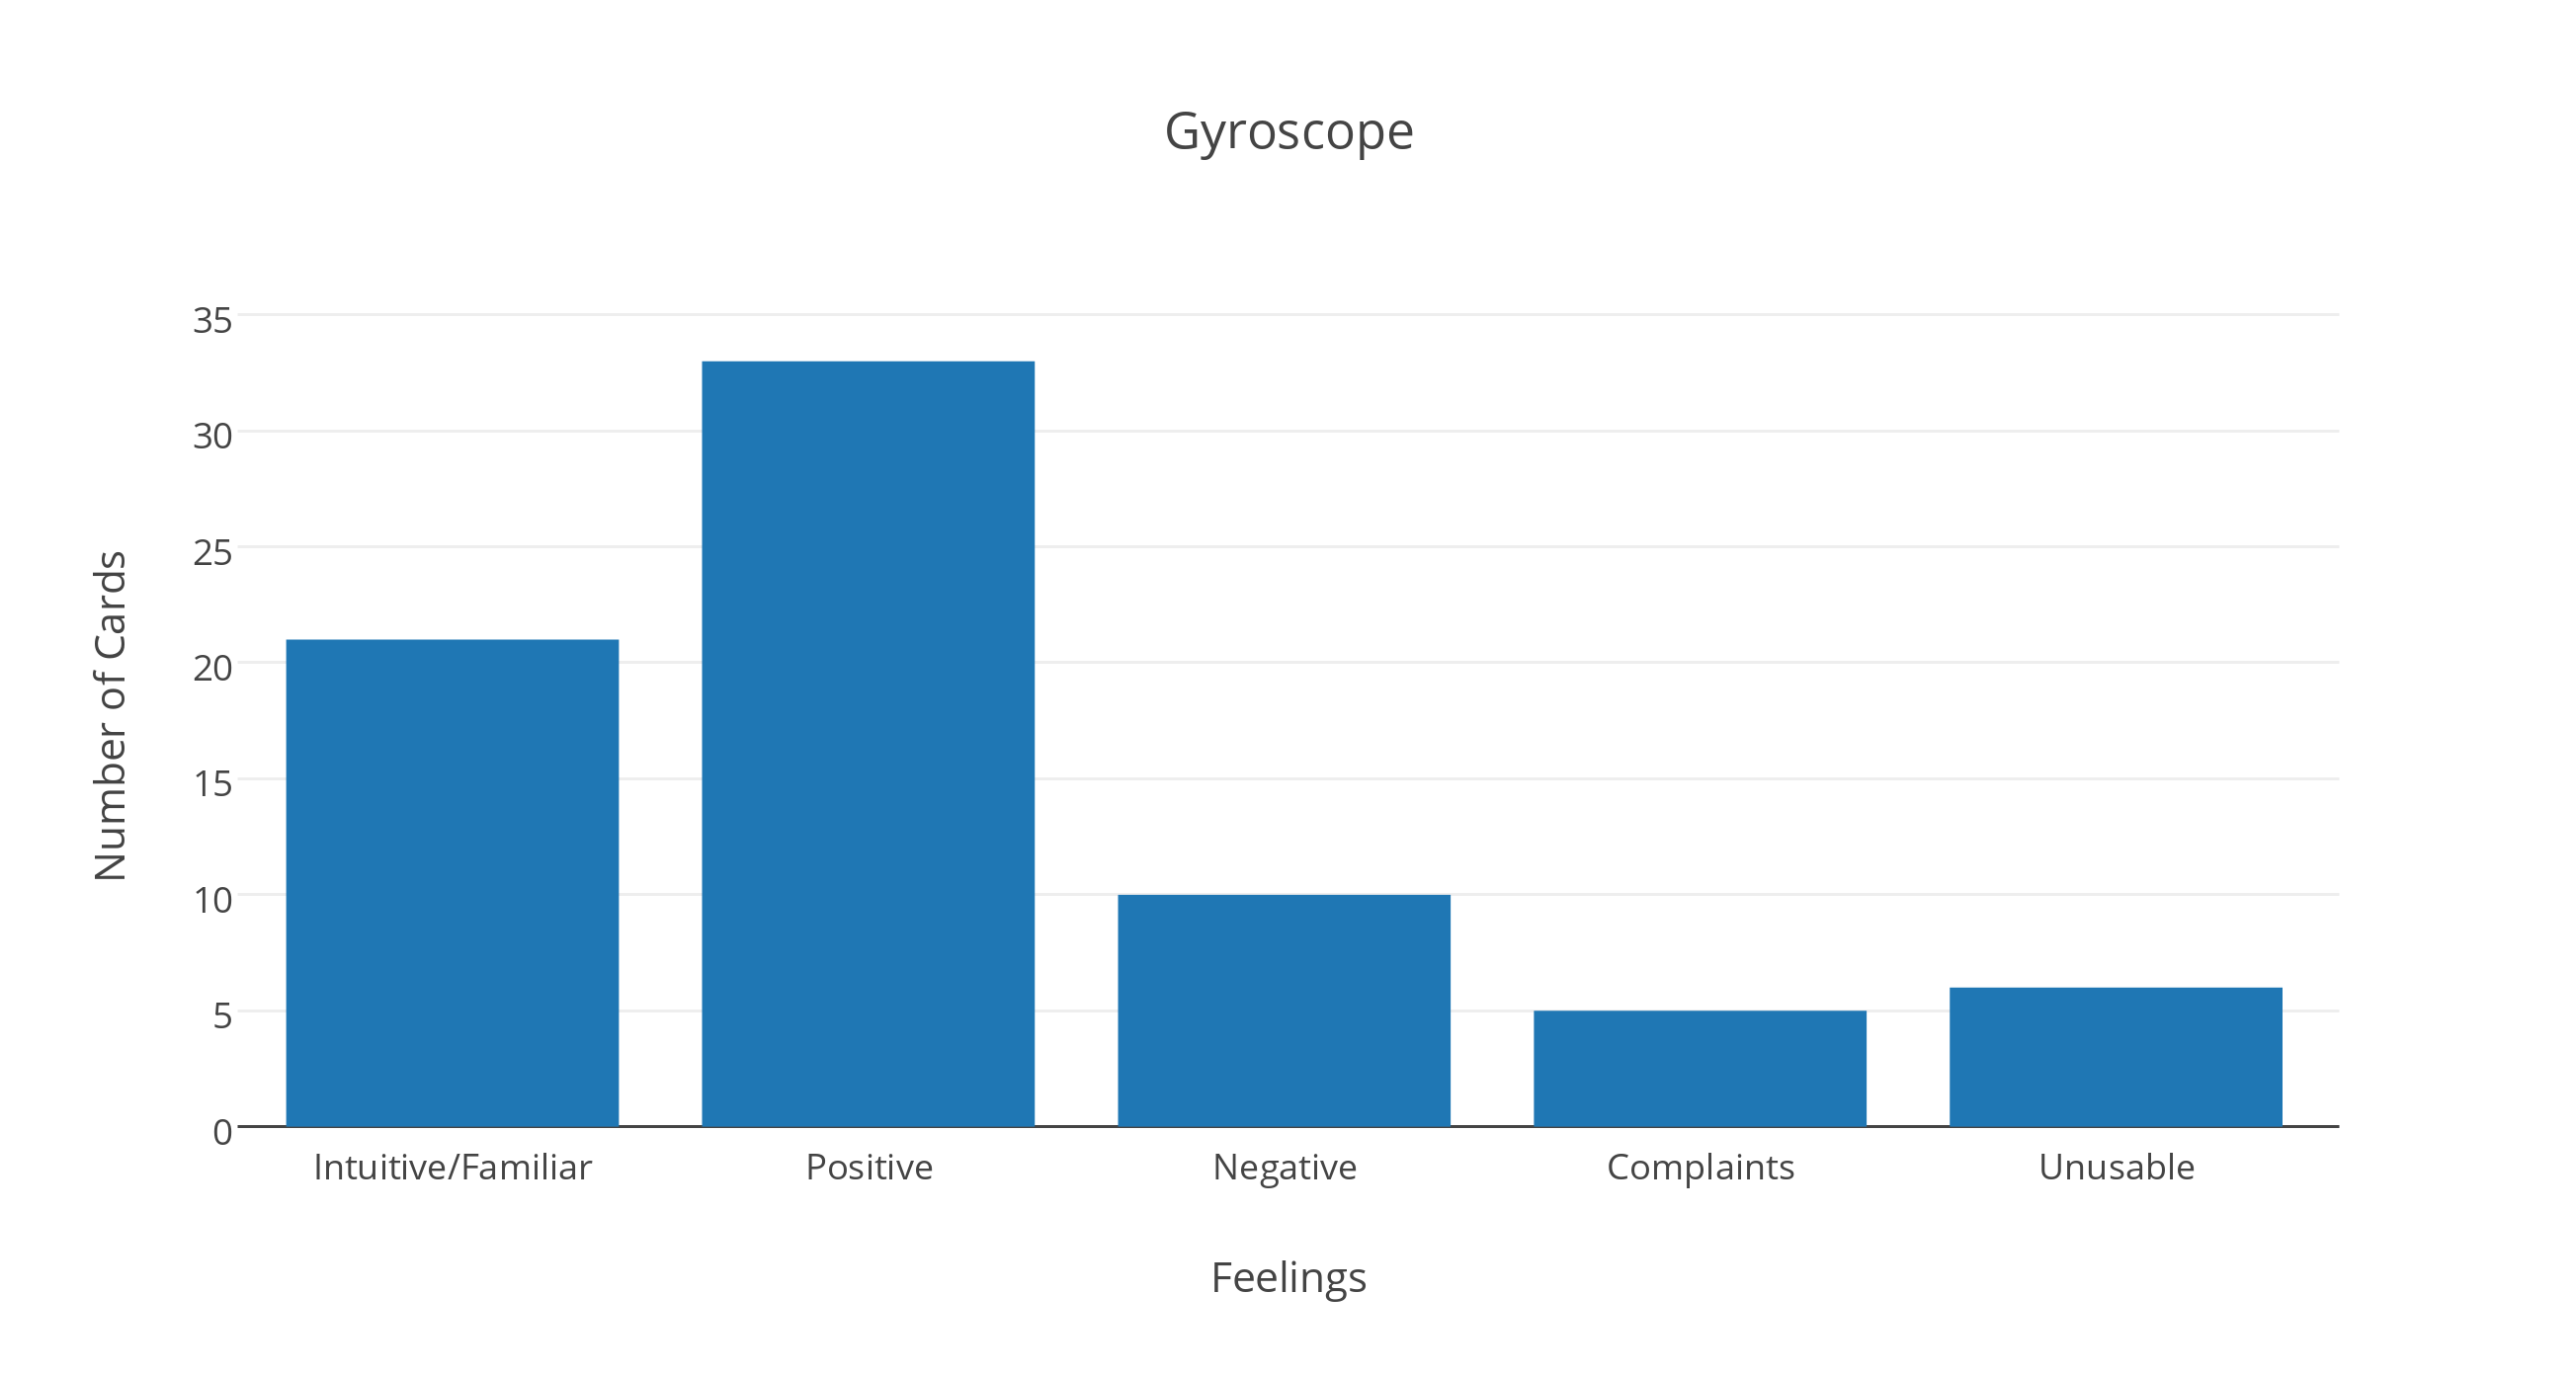
\includegraphics[scale=0.5]{Gyroscope.png}
\caption{Categorisation of the cards for the gyroscope control scheme.}
\end{figure}

The gyroscope turned out to be very intuitive and quite fun for users. It has a small amount of negative feelings and a few complaints. These were mostly based on the fact that you have to turn all the way around and not being able to sit down while using it and that it moved to slow. 
The intuitive cards that were selected showed that the users thought it was nice that their movements was met in a virtual world. Also they thought that it was easy to understand once you have practised a bit. The positive feelings towards the gyroscope was quite clear; it was fun, exciting and friendly. Almost all positive cards had something to with the fact that this was new and that the users had not yet experienced this which made it more attractive.

\begin{figure}[H]
\centering
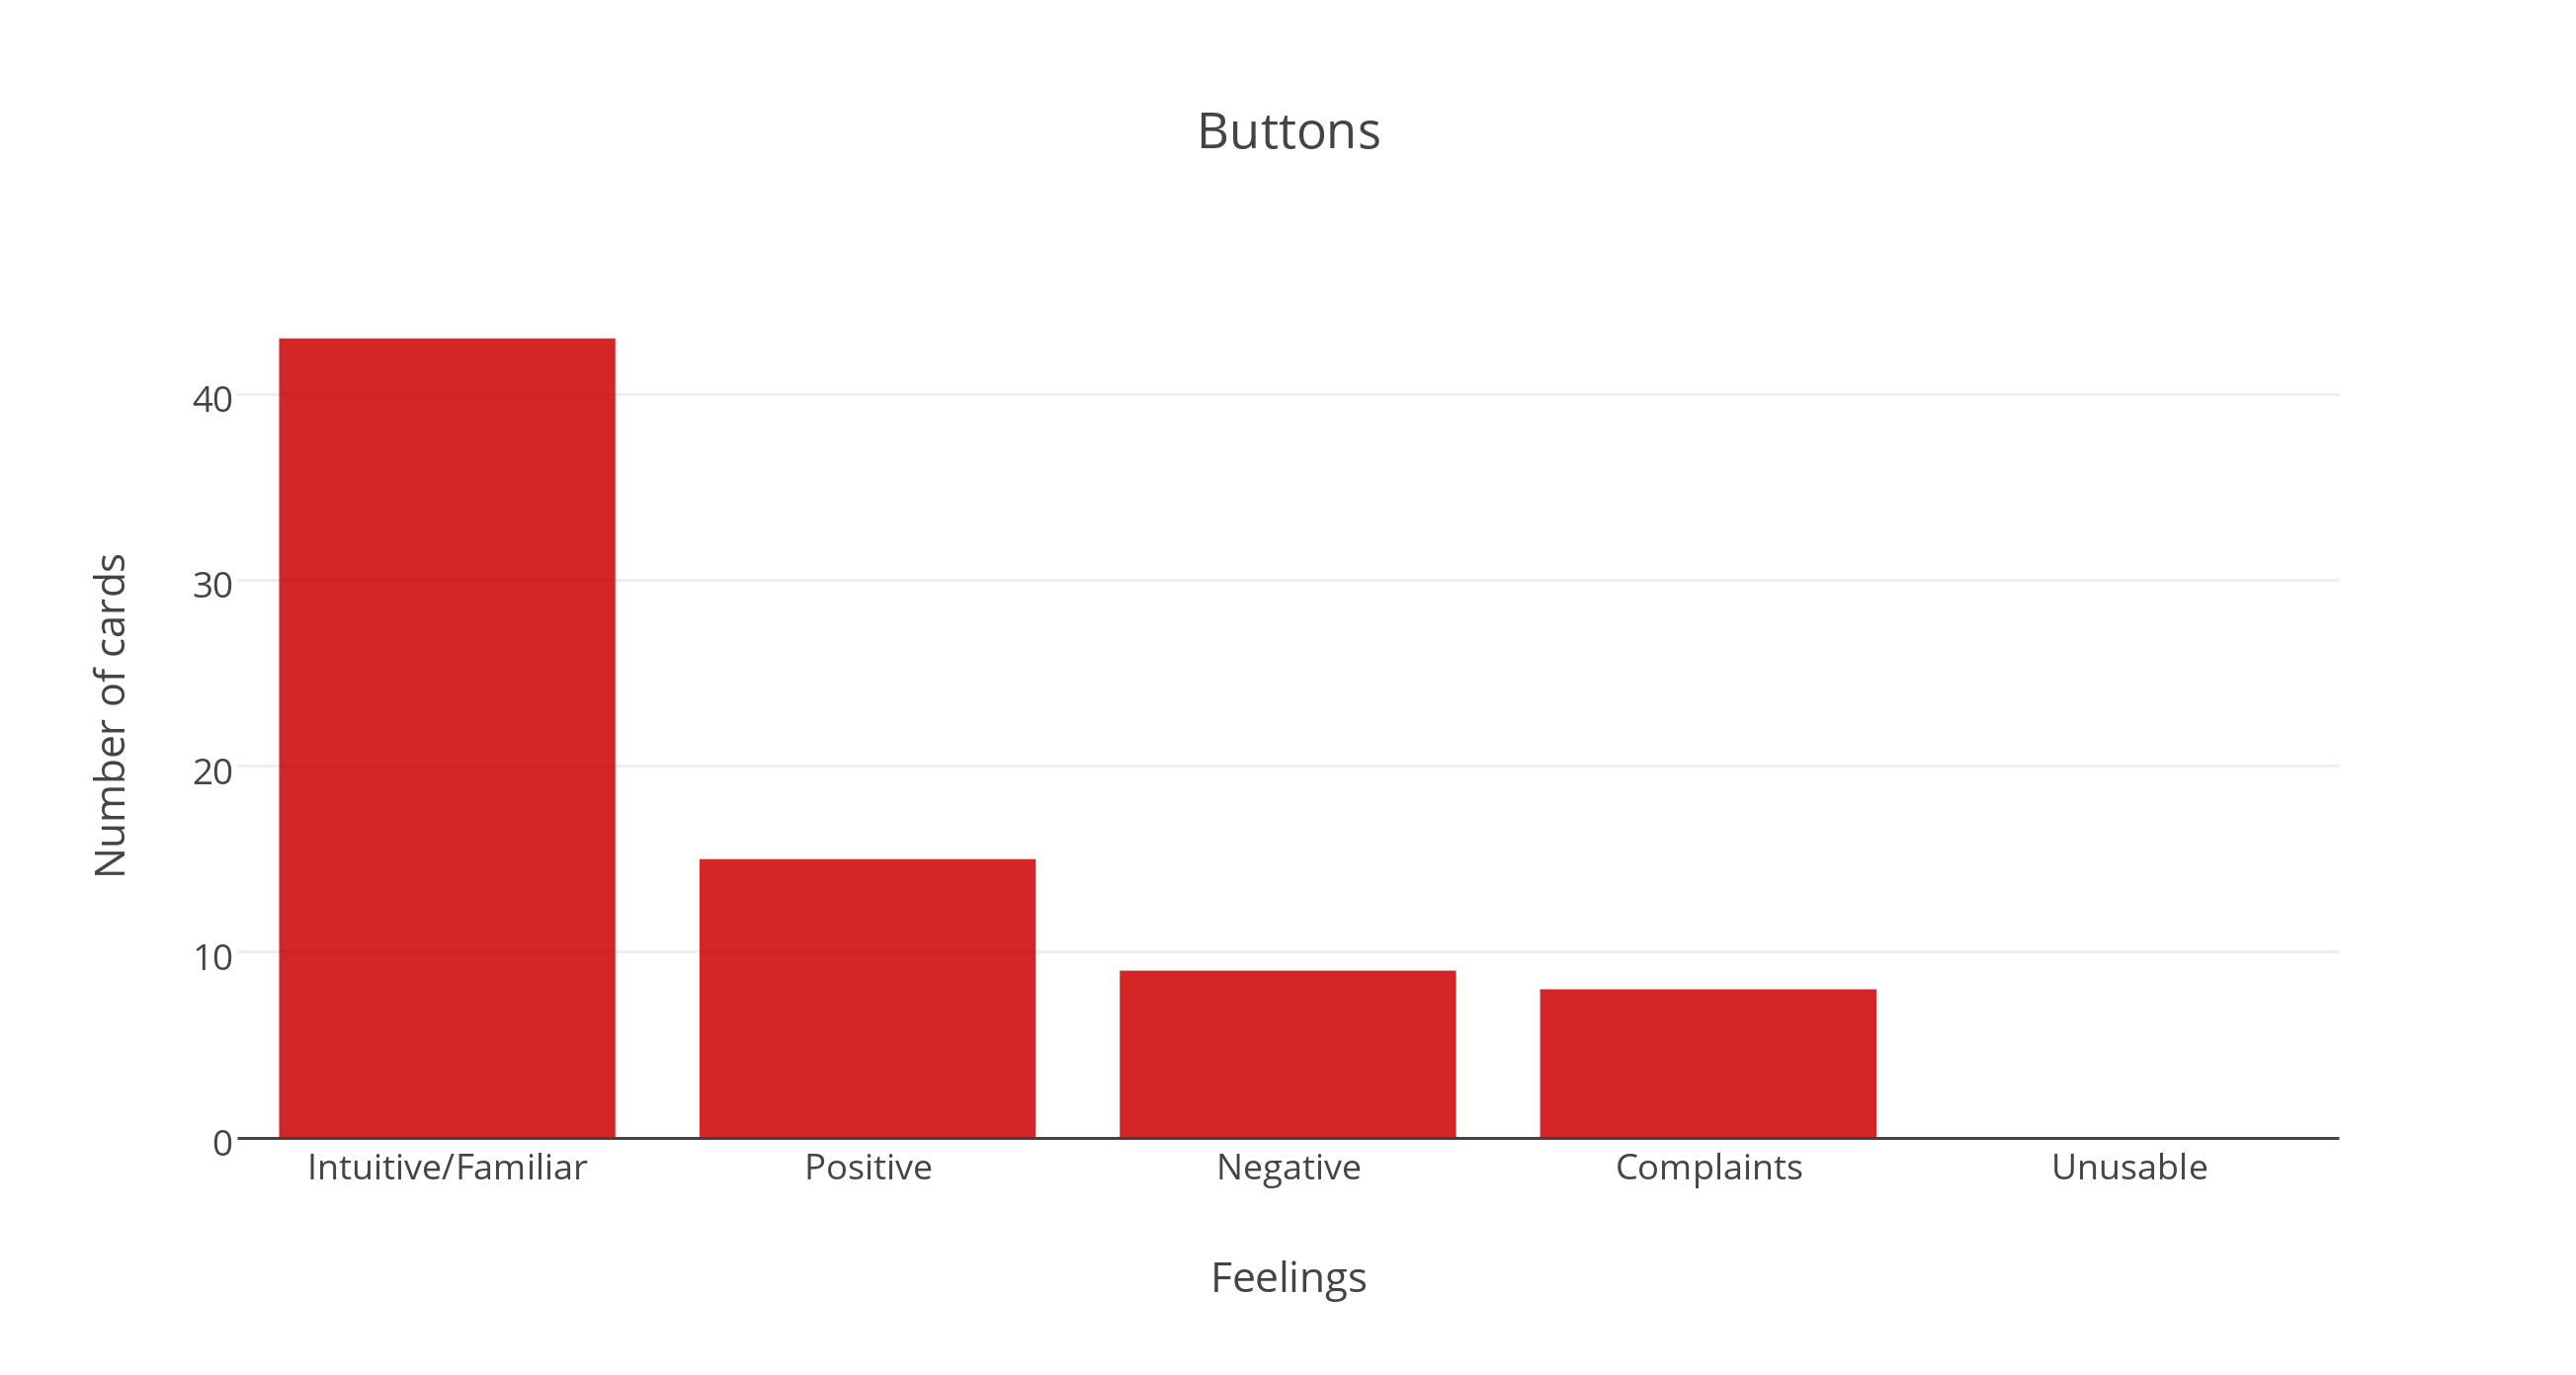
\includegraphics[scale=0.5]{Buttons.png}
\caption{Categorisation of the cards for the button control scheme.}
\end{figure}

The button control scheme has the absolute highest number of intuitive/familiar feelings. This makes sense since it is common for users to use buttons. 
It has about the same amount of negative feelings and complaints as the gyroscope. 5 out of 9 negative cards said dull or boring. The users found that this was too common and had been seen before. It was clearly the most efficient as the intuitive and positive feelings were all directed towards the speed, how easy it was to use and that it was trustworthy. 

\begin{figure}[H]
\centering
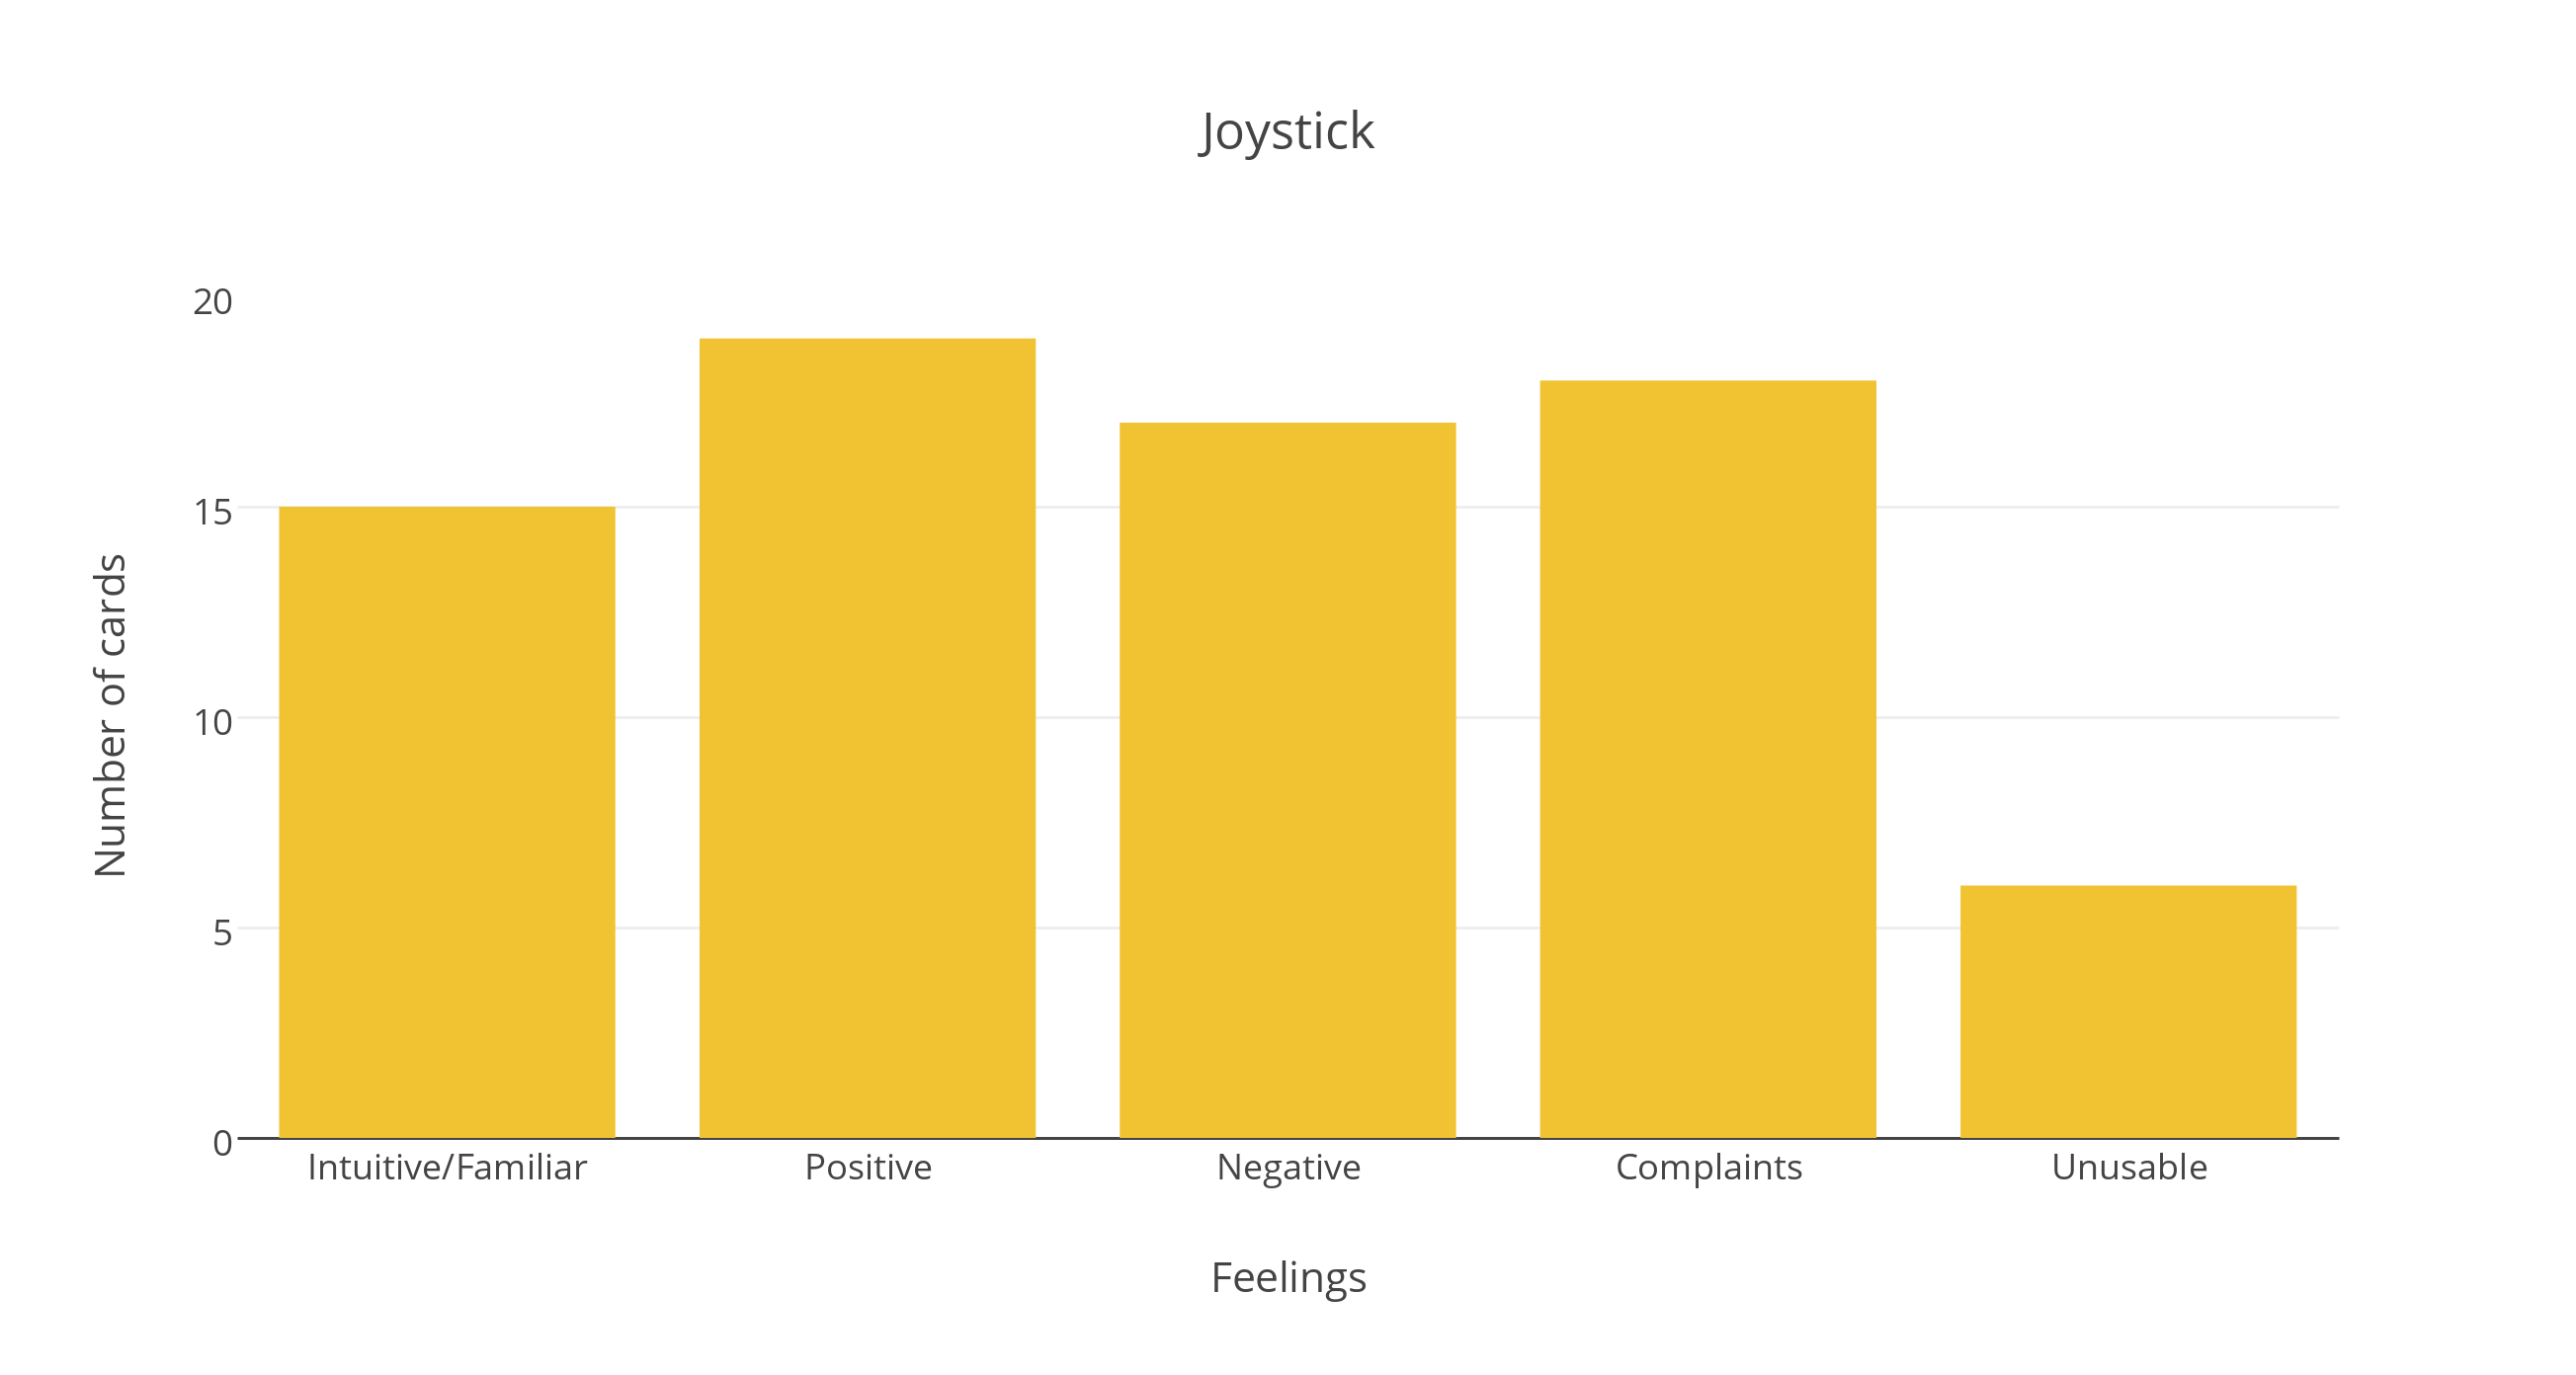
\includegraphics[scale=0.5]{Joystick.png}
\caption{Categorisation of the cards for the joystick control scheme.}
\label{joystickEvaluationResults}
\end{figure}

Lastly, the joystick has a lot of negative feelings and complaints. Even more than it has intuitive/familiar feelings. This clearly shows that the users did not enjoy using this controlling scheme as much as the others and was quite frustrated with it. This could also be provoked by the way this was implemented and the fact that it did not resemble a joystick well enough. The main issues that was pointed out in the negative feelings was that it was frustrating and hard to control. The users commented on the camera the most. 8/18 complaints was directed towards the cameras movement and that the joystick lacked sensitivity. These negative feelings could maybe have been avoided if the implementation had been better. The positive feelings were flexible and creative. The users thought it was fun, once you get to know it. 
The few that did give this control scheme a intuitive/familiar card thought that it was very clear that this was a joystick but still struggled to control it due to the cameras movements.

The joystick might not be as bad as it appears in the bar chart. The main reason for the high number of complaints and negative feelings was that the cameras movement was too sensitive. This could have been prevented by better implementation. So as far as the joystick goes, we will not know if this is the reason for the feedback until we can fix it and test it out once more.


The time from the performance tests was calculated to find the mean and made graphs to demonstrate this. 

\begin{figure}[H]
\centering
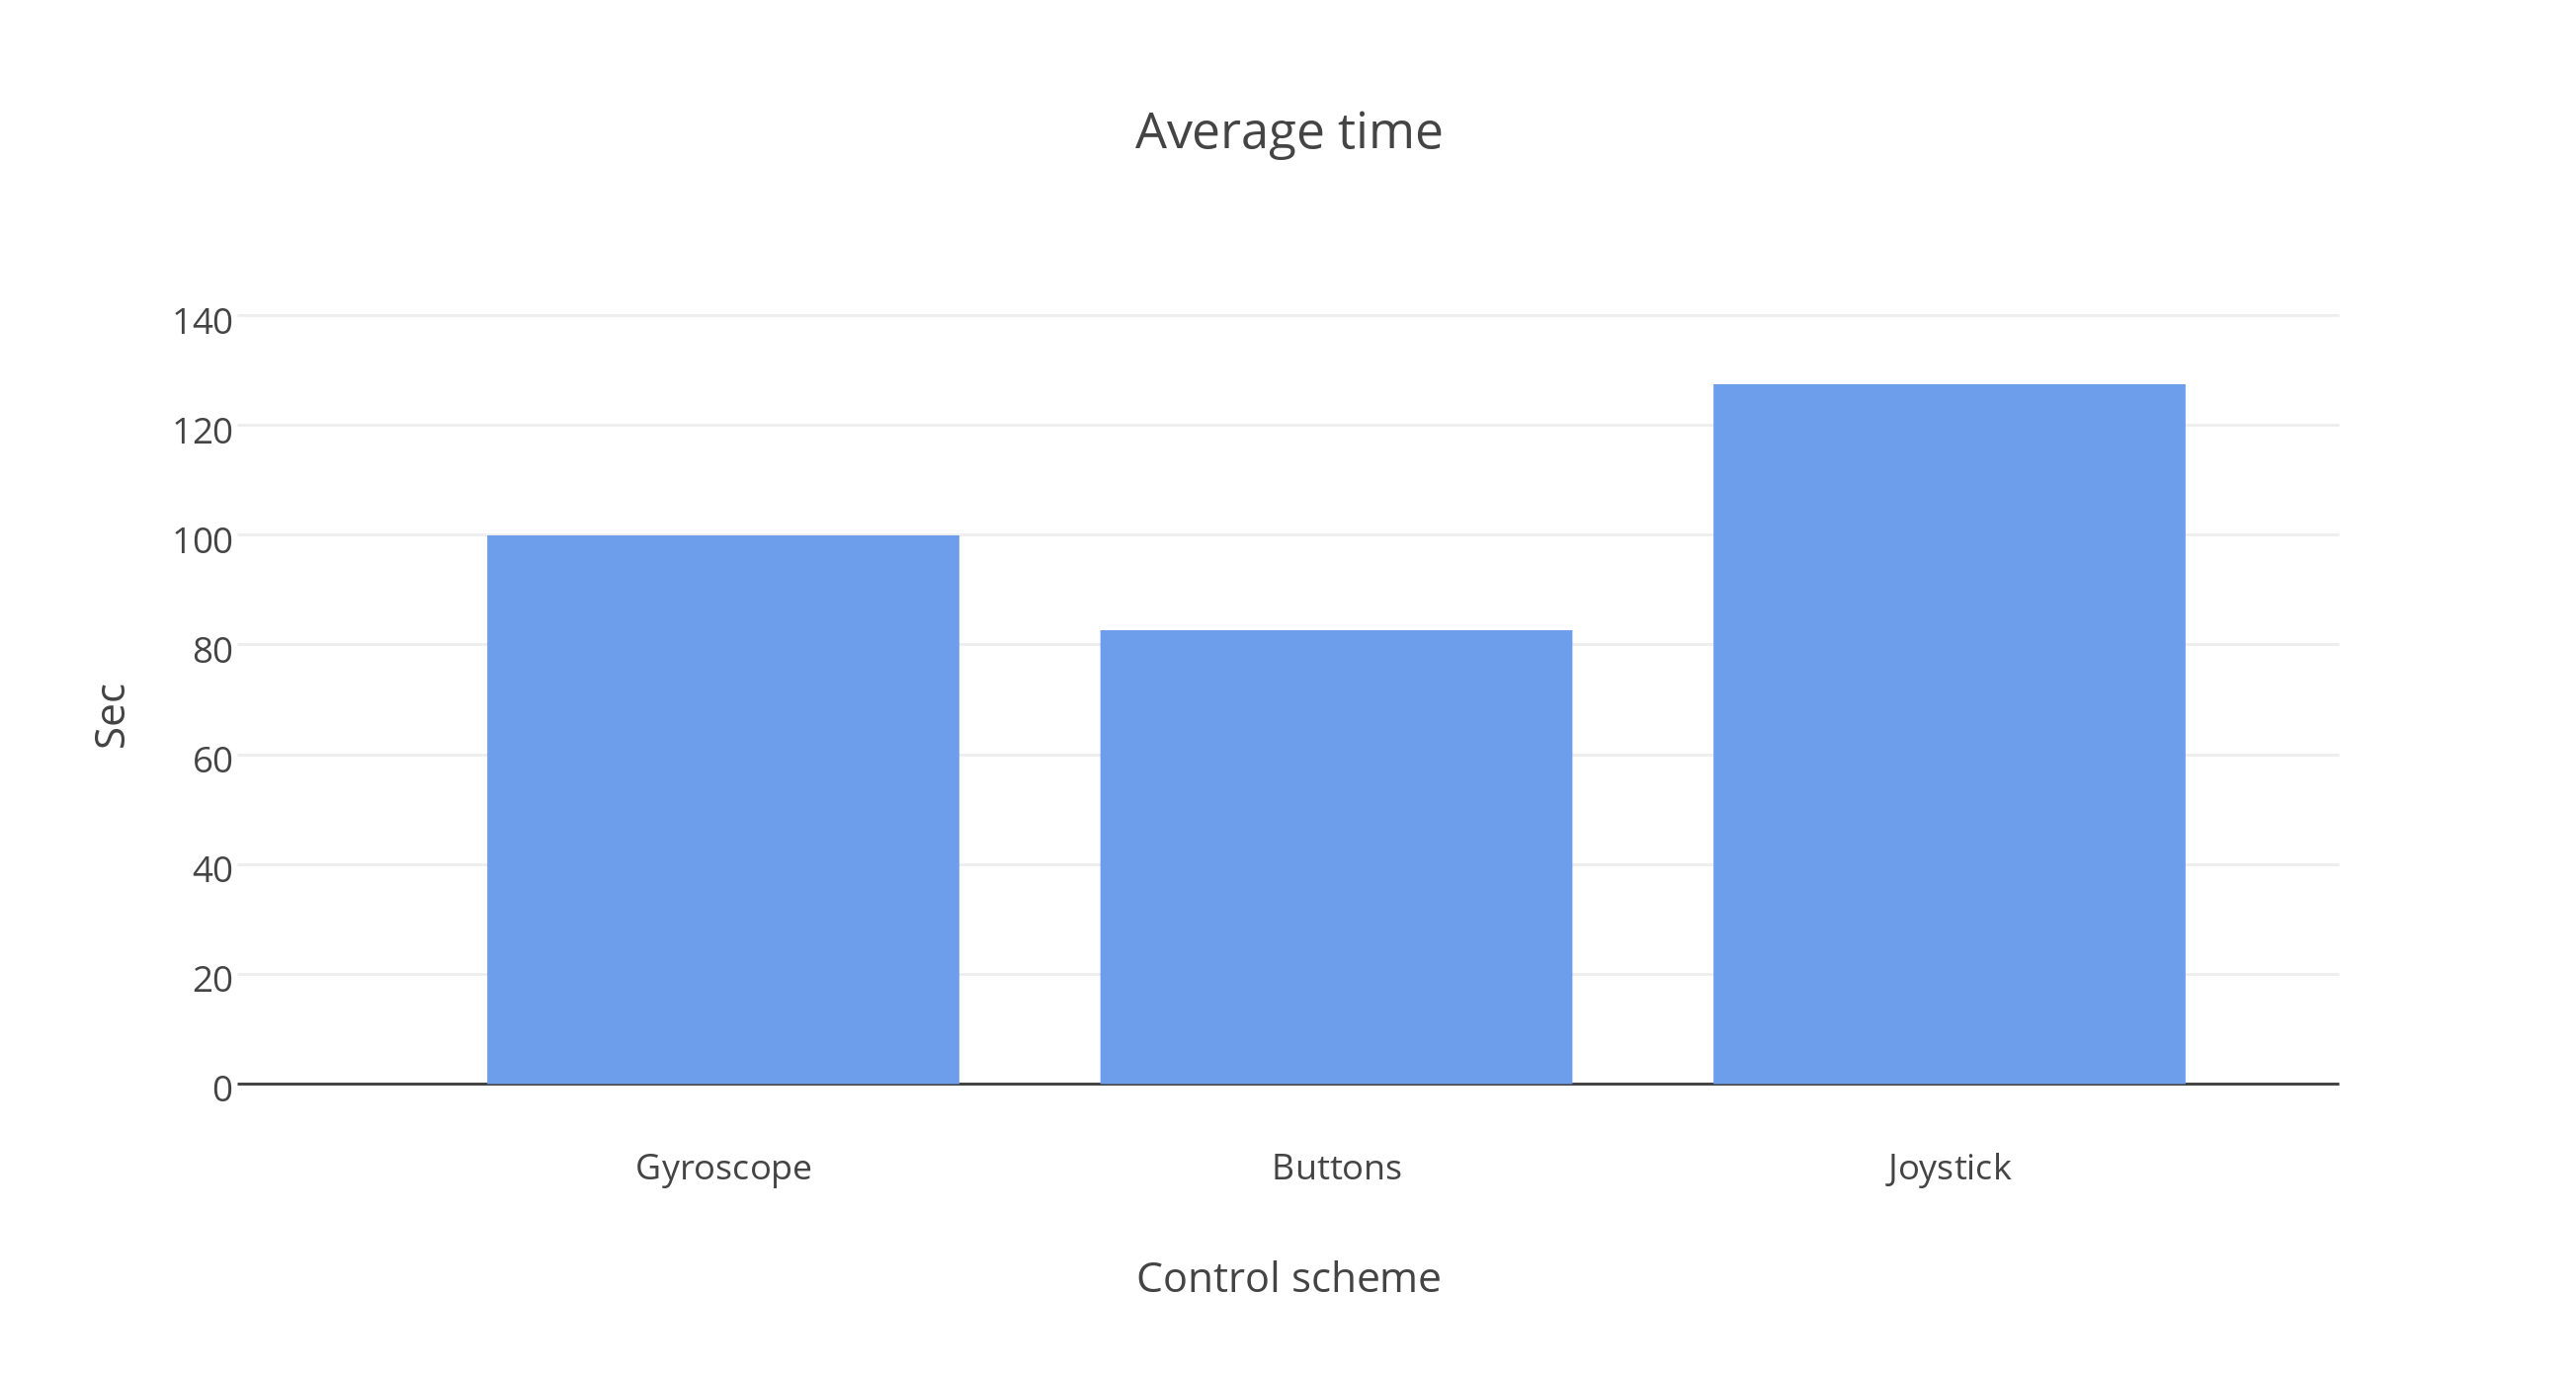
\includegraphics[scale=0.5]{Averagetime.png}
\caption{The average time it took for the participants to complete the level within the different control schemes.}
\end{figure}

It is fairly easy to conclude that the buttons were the most efficient and the joystick the most problematic for our users based on the time alone. But is the buttons the most successful after all?

It shows very clearly that the users had most intuitive/familiar comments about the buttons scheme. And the one they had the hardest time coping with was the joystick. 
Both the performance test and the card sorting test showed that the fastest, most intuitive and most efficient was the buttons scheme. Their emotional response to this was not as we hoped. 
The one controlling scheme the users found the most exciting was the gyroscope. They did have some complaints, but these were mostly based on the fact that there was a learning curve and some technical issues that can be fixed. 

If we were to compare the gyroscope and the button scheme for final conclusion the users had 58 positive feelings/intuitive feelings about the button scheme and 17 negative feelings/complaints. Where as the gyroscope had 54 positive feelings/intuitive feelings and 15 negative feelings/complaints. 

\section{Conclusion of results}

In conclusion, it is now known that the joystick will not be used. 
The final problem statement is interested in making an application that minimizes the knowledge gap using familiarity. (see page: \pageref{FPS})
Also, the user experience section suggest that when people think something is fast, it is good UX. (as mentioned on page: \pageref{EvalConFast}) 
Based on this, it can be concluded that the buttons is the optimal choice for navigation within a 3D environment. Even though the users were more emotionally engaged in the gyroscope, the focus for this app lies within familiarity and not excitement. And even though the negative cards that were chosen in the card sorting suggested that the users found this boring, it still sets the bar high with 43 cards chosen on familiarity and intuition.
 

